\documentclass[11pt,a4paper]{article}
\usepackage[T1]{fontenc}
\usepackage[utf8]{inputenc}
\usepackage{lmodern,microtype}
\usepackage[margin=25mm,headheight=14pt]{geometry}
\usepackage{amsmath,amssymb,amsthm,mathtools,stmaryrd}
\usepackage{booktabs,longtable,tabularx,array}
\usepackage{xcolor,graphicx,tikz}
\usetikzlibrary{positioning,arrows.meta}
\usepackage{listings,enumitem,fancyhdr,etoolbox,needspace}
\usepackage[hyphens]{url}
\usepackage[colorlinks=true,linkcolor=blue!40!black,citecolor=blue!40!black,urlcolor=blue!40!black]{hyperref}
\usepackage{bookmark}
\definecolor{ink}{HTML}{18354A}
\definecolor{pale}{HTML}{F2F5F7}
\definecolor{accent}{HTML}{226377}
\lstset{basicstyle=\small\ttfamily,columns=fullflexible,keepspaces=true,
 breaklines=true,showstringspaces=false,frame=single,rulecolor=\color{black!15},
 backgroundcolor=\color{pale},xleftmargin=5pt,xrightmargin=5pt,
 framesep=6pt,aboveskip=12pt,belowskip=12pt,tabsize=2}
\BeforeBeginEnvironment{lstlisting}{\par\noindent\begin{minipage}{\linewidth}}
\AfterEndEnvironment{lstlisting}{\end{minipage}\par}
\widowpenalty=10000
\clubpenalty=10000
\newcommand{\code}[1]{\texttt{\detokenize{#1}}}
\newcommand{\N}{\mathbb N}\newcommand{\Z}{\mathbb Z}
\newcommand{\Q}{\mathbb Q}\newcommand{\R}{\mathbb R}
\newcommand{\E}{\mathcal E}\newcommand{\Guard}{\mathsf{Guard}}
\newcommand{\den}[1]{\llbracket #1\rrbracket}
\newcommand{\Noema}{\textsc{Noema}}
\newcolumntype{P}[1]{>{\raggedright\arraybackslash}p{#1}}
\newcolumntype{Y}{>{\raggedright\arraybackslash}X}
\newtheorem{proposition}{Proposition}[section]
\newtheorem{definition}[proposition]{Definition}
\theoremstyle{remark}\newtheorem{example}[proposition]{Example}
\setlist{itemsep=3pt,topsep=6pt}
\setlength{\parskip}{5pt}
\setlength{\parindent}{0pt}
\setlength{\emergencystretch}{2em}
\pagestyle{fancy}\fancyhf{}
\fancyhead[L]{\small\color{ink}\Noema: reasoning and certified computation}
\fancyhead[R]{\small Second-round proposal}
\fancyfoot[C]{\thepage}
\hypersetup{pdftitle={Noema: Mathematical Objects, Scoped Relations, and Certified Computation},pdfauthor={GPT-6 Pro, prepared for Vladimir Reshetnikov},pdfsubject={Second-iteration proof-language design grounded in ProveIt, Leant, and Brainstorm}}
\begin{document}
\begin{titlepage}
\vspace*{18mm}
{\large\color{accent} PROOF LANGUAGE DESIGN\quad /\quad ITERATION TWO}\par
\vspace{12mm}
{\Huge\bfseries\color{ink} Noema}\par
\vspace{5mm}
{\LARGE Mathematical Objects, Scoped Relations,\par and Certified Computation}\par
\vspace{10mm}
{\large A human-scale language over Lean,\par with a proof-producing computer algebra layer}\par
\vspace{13mm}
\textbf{Prepared for Vladimir Reshetnikov}\par
GPT-6 Pro\par
5 September 2026 (Pacific time)
\vspace{12mm}
\begin{abstract}
A mathematician alternates between choosing objects, recognizing a structure, applying a theorem, and calculating. A useful proof language should support that entire cycle, not merely replace tactic names with English. This article proposes \Noema, a conservative extension of the common architecture identified by the two Brainstorm syntheses: Lean remains the checking foundation; mathematical choices remain visible; routine consequences acquire retained evidence.

The principal extension is a \emph{contract calculus for symbolic computation}. A computation returns an object together with the precise relation it establishes, its domain and precision, and checkable evidence. Equality, equality on an open set, agreement of finitely many coefficients, and numerical enclosure are different results, not different displays of one equality. Definition packages connect mathematical specifications to computational representations through proved interfaces. A verified reference algorithm or a verified certificate checker supplies the logical basis of each computational service; an external CAS or Leant may search without becoming an oracle.

The proposal develops surface syntax, dependent obligation interfaces, guarded view composition, a two-path CAS architecture, a Leant integration contract, six mathematical case studies, and explicit answers to the syntheses' next-round questions. A small accompanying Python experiment exercises 25 certificate-boundary tests with exact rational arithmetic. It is not a formally verified implementation. The proposed language has not been implemented or compiled, and no new Lean or Leant execution is claimed.
\end{abstract}
\vfill
{\small\color{ink}\textbf{Design thesis}\quad Make the mathematical choice explicit; make the computation's meaning part of its type; reconstruct and retain the evidence.}
\end{titlepage}
\begingroup\small\setlength{\parskip}{0pt}
\tableofcontents
\endgroup
\clearpage

\section{The proposal in one mathematical session}\label{sec:session}
Suppose a mathematician is studying the real root of
\[
 p(x)=x^3-x-1
\]
in the interval $[1,2]$. The mathematical argument is short: the signs at the endpoints differ, and $p'(x)=3x^2-1\geq2$ on the interval. An exact computation then gives a much narrower rational enclosure. The proposed surface could read:
\begin{lstlisting}
object p : Polynomial Rational := X^3 - X - 1

claim unique_root : exists unique r in [1,2], p(r) = 0
proof
  calculate p(1) = -1 and p(2) = 5 by exact arithmetic
  calculate derivative p = 3*X^2 - 1 by polynomial calculus
  have derivative p >= 2 on [1,2] by ordered polynomial algebra
  conclude by continuous bracketing and strict monotonicity

noncomputable select r with root_spec from unique_root
  by classical choice
enclose r in [331/250, 53/40]
  by monotone bracketing using root_spec
\end{lstlisting}
Every command above is \emph{design pseudocode}, not an existing Lean extension. Its intended interface is nevertheless precise. The polynomial object is distinct from its real-valued evaluation. The root is selected by a specification, not replaced with a floating-point number. This particular real-valued selection explicitly uses classical choice; it is not an executable real-root algorithm. A computational algebraic-number representation requires a separately certified construction. The enclosure is an inequality theorem about that same root. The continuity and monotonicity obligations belong to named theorems. Rational evaluations are exact computations, not empirical evidence that a root probably exists.

This session suggests the essential unit of the language:
\[
 \boxed{\text{object or claim}\; +\;\text{requested relation}\; +\;
        \text{mathematical method}\; +\;\text{retained evidence}.}
\]
A user can work forward from an expression, as in a CAS, or backward from a proposition, as in a proof assistant. These are two entry points to the same typed calculation, not two systems with incompatible notions of truth.

\subsection{What should become shorter}
The source should normally expose the root interval, the derivative argument, the index substitution in a sum, the induction invariant, or the choice of a formal rather than analytic interpretation. It should not normally require an author to spell out every cast, conjunction projection, reassociation, theorem argument, or proof that an index belongs to an interval already being traversed. Whether a premise is routine depends on the local problem: a nonzero denominator can be immediate in one proof and its main theorem in another.

Concision is therefore not unrestricted omission. It is \emph{the removal of repeatedly reconstructible work after its meaning has been fixed}. In particular, ``the CAS simplified it'' is not an adequate mathematical reason. ``Cancel the nonzero factor $x-1$'' can be adequate, provided the scope supplying $x\ne1$ and the checked cancellation contract are accessible.

\subsection{What is inherited, and what is being added}
The two syntheses already articulate most of the required proof architecture~\cite{synthesis,blueprints}. This article does not claim to invent typed steps, proof reflection, controlled natural language, or certificate-producing computation. Its contribution to the campaign is a specific integration design and a set of decisions that can be implemented and tested.
\begin{tabularx}{\textwidth}{@{}P{.25\textwidth}Y@{}}
\toprule
Status & Design content \\
\midrule
Adopt from round one & Lean host; fixed targets; scoped dependent obligations; theorem-backed methods; all-assertion coverage; separate discovery and replay; fair Lean baselines.\\
Make more specific & Stable method wrappers; exact candidate-origin checking; an explicit composition rule for guarded views; separate proof, construction, and approximation results; service-independent publication.\\
New organizing emphasis & Relation-typed symbolic calculations; precision as a logical contract; specification-first definition packages; computation-driven proof development sharing one object model.\\
Test, rather than assume & Whether the new surface helps authors or readers; whether a verified CAS reduces total effort; whether definition packages amortize their cost.\\
\bottomrule
\end{tabularx}

\section{What the source material actually establishes}\label{sec:reading}
\subsection{A close reading of the two syntheses}
\emph{Mathematical Ideas, Checked Evidence} identifies six common commitments across Contour, Loom, MathStep, MPL, Mosaic, Motive, Outline, Reason, and Spine. It distinguishes target fidelity, logical evidence, document coverage, and method conformance, and insists that explanatory quality remains a separate empirical question. Its strongest practical recommendation is to compare two frontends over one infrastructure rather than build nine languages~\cite{synthesis}.

\emph{Nine Blueprints for a Mathematician's Proof Language over Lean} provides a finer comparison, a lexical corpus audit, an inventory of existing Lean mechanisms, and a detailed discussion of definitions and Leant. Its most useful simplification is that many logical method contracts should be ordinary theorem types with role annotations. Its warning about ``accounting'' is also valuable: obtaining a consequence is not the same as retaining an intelligible record of the inputs, guards, and method that obtained it~\cite{blueprints}.

The revised reports have already incorporated criticisms of one another. In particular, they now distinguish semantic notices from real proof obligations, tactic-text freezing from term-level evidence, and heuristic source classification from measured removable work. It would be a mistake to write a second-round proposal against their superseded versions.

I adopt the following resolutions of their remaining disagreements. The language is initially \emph{both a small input form and a rendered view of ordinary Lean}; the shared typed representation is the product. Named transformations require method conformance, while an explicitly open \code{prove} request may use any permitted proof. Definitions enter early through a few specification templates, not a new universal definition language. Leant remains a Haskell service behind a Lean-owned boundary. An implementation may stop at a library and document view if new syntax produces no additional benefit.

\subsection{Four actual ProveIt examples}
The source inspection for this article used the public revision recorded in Appendix~\ref{app:sources}; it is not a rerun of the syntheses' local working-tree review.
\begin{longtable}{@{}P{.27\textwidth}P{.34\textwidth}P{.31\textwidth}@{}}
\toprule
Inspected module & What the source does & Design requirement \\
\midrule\endhead
\path{BinomialInversion.lean} & Reindexes an integer kernel sum, transports binomial products through casts, then reuses a triangular-kernel calculus. Public inversion works in an additive commutative group. & Make the map and kernel identity visible; preserve module-level generality.\\
\texttt{Autonomous\allowbreak{}Iterated\allowbreak{}Deriv.lean} & Builds neighborhood equality from an induction identity on an open set, then applies derivative congruence and the chain rule. & Local equality and range-local differentiability must survive the shorter surface.\\
\path{AbelPolynomialSeries.lean} & Applies formal Lagrange inversion, proves substitution admissibility, and transports rational scalar identities into a commutative rational algebra. & Do not replace an arbitrary solution by a canonical one or strengthen the coefficient algebra to a field.\\
\path{FloorSqrtSum.lean} & Proves a rational formula, establishes exact division and a subtraction bound, then transfers the result to natural numbers. & Guarded transport must retain truncation and divisibility semantics.\\
\bottomrule
\end{longtable}
These are direct static observations~\cite{binomial,ode,abel,sqrt}. Some public corollaries are already extremely short. The relevant comparison is not ``long Lean versus short pseudocode,'' but equally equipped Lean versus a surface that may better expose mathematical choices.

\subsection{Three cautions about the evidence}
First, the second synthesis reports 90,637 classified tactic-like entries in 1,004 files, with 32.3\% placed in families suggested for reconstruction. These are the report's lexical measurements, not measurements made here and not a forecast of savings. The result motivates sampling analysis, casts, and coefficient calculations; it does not establish how many can be solved automatically~\cite[section 3]{blueprints}.

Second, a translation's safety flags or an empty list of abstracted nodes are useful diagnostics, but are not themselves a formally checked adequacy theorem. This distinction matters when transferring a negative search result back to Lean. The implementation should be stricter than the second synthesis's occasional description of the safety bit as the general adequacy mechanism: require an actual proof at the original target, or a checked certificate composed with a proved translation theorem.

Third, source text without \code{sorry} does not establish successful compilation, an acceptable transitive axiom inventory, or intended statement meaning. Likewise, reading a test fixture does not mean that its tests were run. The article's own execution claims are confined to the explicitly described Python experiment in Section~\ref{sec:experiment}.

\section{The language: few commands, substantial mathematical contracts}\label{sec:language}
\subsection{Three kinds of author request}
\Noema\ separates requests whose mathematical effects differ.

\textbf{Establish a claim.} A \code{have}, \code{show}, or \code{prove} request fixes a proposition in its actual dependent context. A proof-only provider may change the evidence, but not the proposition or any previously accepted object.

\textbf{Transform an expression.} A \code{calculate} or \code{transform} request names an input, a desired output form or target expression, and a relation. An output is accepted only with evidence of that relation. Global equality is the default; a local domain, finite precision, or error tolerance must be explicit when it weakens the requested conclusion.

\textbf{Introduce an object.} A \code{construct} request fixes a type and a specification; the result contains both the object and evidence that it satisfies the specification. \code{obtain} instead eliminates an existing existential theorem in a permitted scope. A \code{define} command introduces a fixed construction, not a theorem that a solver may reinterpret. Noncomputable \code{select} explicitly uses an allowed choice principle; it is distinct from scoped existential elimination and from an executable construction.

An enclosure is a transformation or assertion in an inequality relation, not a fourth foundational mechanism. Separate surface wording makes its weaker output unmistakable:
\begin{lstlisting}
calculate E = F by polynomial algebra
calculate f = g on U by guarded rational algebra
calculate F == G mod t^N by formal series arithmetic
enclose value in [a,b] by certified interval arithmetic
construct r : Real satisfying 0 < r and r^2 = a
  by positive-root construction
\end{lstlisting}
A command that requests equality cannot quietly return an enclosure. A command that constructs one root cannot quietly claim to enumerate every root.

\subsection{Proof structure remains familiar}
The core retains named assertions, calculations, scoped cases, existential elimination, reductions, and induction. For example:
\begin{lstlisting}
proof
  cases n < j
  case true:
    conclude by empty interval
  case false:
    obtain m : Nat with n = j + m by natural arithmetic
    reindex target sum by i |-> j + i from [0..m] to [j..n]
    calculate each summand by binomial product identity
    conclude by alternating binomial row
\end{lstlisting}
The example gives a mathematical plan, not merely the final target to an unrestricted solver. The reindexing method must prove the actual map's coverage and summand correspondence. If that plan fails but another proof succeeds, the alternative is proposed as an edit to the plan rather than installed behind the old explanation.

Induction is similarly explicit about the motive whenever it is not the visible goal. A proposed strengthening of the induction invariant is a plan change requiring review, even when the public theorem is unchanged. ``Similarly'' can only instantiate a registered checked pattern with fresh obligations. ``The remaining cases'' must expand the actual recursor's remaining constructors and retain coverage information. None of these phrases means permission to omit a difficult case.

\subsection{Stored source is controlled; drafting need not be}
Initially, formulas reuse Lean expressions and a small collection of fixed notation profiles. A natural-language assistant may draft a controlled block, retrieve a theorem, or suggest a more useful intermediate identity. Its output is an editable proposal. It may not settle a missing branch, domain, coefficient structure, or quantifier order by searching for whichever interpretation proves easiest.

Controlled natural language is not new: Verbose Lean provides a Lean-based setting for teaching the reading and writing of traditional proofs~\cite{verbose}. The present design has a different primary emphasis, namely certified symbolic work on mathematical objects. Whether its surface improves advanced proof development remains to be measured.

The accepted syntax tree stores stable claim identities. A reader-facing phrase such as ``the preceding inequality'' renders a resolved reference; inserting a new sentence does not silently change its target. An explicit retargeting edit shows a mathematical difference. Copying a proof block creates fresh identities and rechecks its imported references and scopes.

\subsection{Permission to omit is local and bounded}
A profile contains a small, versioned portfolio of routine methods. For an interval sum, membership hypotheses can feed arithmetic immediately. For a rational-algebra calculation, scalar maps and polynomial normalization can be selected without searching unrelated analysis lemmas. Premises involving domination, nontrivial branch selection, or an unproved regularity property remain visible unless an already accepted local theorem supplies them.

This is not a permanent classification of propositions as trivial. Roles describe how a particular method invocation treats a binder. The author can promote a generated obligation into a named claim; a reader can expand it. The same proposition may be collapsed in one context and central in another.

The first implementation should not offer a global ``obvious'' command with unspecified search. An open proof request carries a bounded provider policy. A named method carries its own theorem and permitted discharge policy. Every timeout leaves an identifiable open obligation, not an unexplained failure of the whole document.

\section{Relation-typed calculations}\label{sec:relations}
\subsection{Why ordinary equality is not enough}
A computer algebra session often moves among formulas, functions, truncated expansions, and numerical approximations. A proof assistant must distinguish their meanings. \Noema\ therefore makes the relation being established a first-class component of a calculation.
\begin{longtable}{@{}P{.23\textwidth}P{.40\textwidth}P{.29\textwidth}@{}}
\toprule
Relation & Exact meaning & Forbidden automatic promotion \\
\midrule\endhead
Equality & $a=b$ in a fixed type. & Changing the type, operations, or instance.\\
Equality on $U$ & $\forall x\in U,\ f(x)=g(x)$. & Equality outside $U$.\\
Equality near $x$ & $f=g$ eventually along $\mathcal N(x)$. & A global function identity.\\
Coefficient agreement & $[t^k]F=[t^k]G$ for every $k<N$. & Equality of the full series.\\
Enclosure & $a\leq v\leq b$ in a specified ordered type. & $v=(a+b)/2$, or a strict endpoint inequality.\\
Error bound & $d(v,w)\leq\varepsilon$ in a specified metric. & Exact equality unless the bound permits it by theorem.\\
Representation relation & $V(a,b)$ with an explicit meaning-preserving operation. & Equality of the representatives themselves.\\
\bottomrule
\end{longtable}
These relations do not form one convenient universal lattice. Equality on sets has restrictions; filters have their own order; numerical errors compose through estimates; series precision interacts with differentiation. The implementation should register actual implication, congruence, and composition theorems, not invent a universal ``weaker than'' coercion.

\subsection{Composition is a theorem application}
Suppose a relation-composition theorem has type
\[
 c:\ \forall a\,b\,d,\ R(a,b)\to S(b,d)\to T(a,d).
\]
A calculation chain may apply $c$ after its middle objects and structures are resolved. Mixed equality/inequality chains are a familiar special case. Domain restrictions and analytic premises are part of the particular theorem, not extra informal annotations.

For example, if $f=g$ on $U$ and $g=h$ on $V$, then $f=h$ on $U\cap V$. To conclude equality on a previously requested $W$, the method owes $W\subseteq U\cap V$. It may not shrink $W$ silently. The UI should show ``the requested domain is larger than the certified domain'' rather than automatically proving a weaker theorem.

For distances, the triangle inequality gives
\[
 d(a,b)\leq\varepsilon,\quad d(b,c)\leq\delta
 \quad\Longrightarrow\quad d(a,c)\leq\varepsilon+\delta.
\]
Transport through an $L$-Lipschitz function changes the error to $L\varepsilon$. The Lipschitz theorem and the relevant domains are required inputs. A display that rounds $L\varepsilon$ upward is a presentation of a proved bound; one that rounds it downward changes the claim.

\subsection{Finite precision has an exact algebraic meaning}
For formal power series over a commutative ring, write
\[
 F\equiv_N G\quad\Longleftrightarrow\quad
 \forall k<N,\ [t^k]F=[t^k]G.
\]
The relation records exact agreement of finitely many coefficients. It is not analytic big-$O$ notation, although there are settings in which additional theorems relate the two.

\begin{proposition}[Basic precision contracts]\label{prop:precision}
If $F\equiv_N G$ and $H\equiv_N K$, then
\[
 F+H\equiv_N G+K,\qquad FH\equiv_N GK.
\]
If $F\equiv_{N+1}G$, then $F'\equiv_N G'$. If $F\equiv_N G$ for every $N\in\N$, then $F=G$.
\end{proposition}
\begin{proof}
Addition is coefficientwise. The coefficient of degree $k$ of a product uses only coefficients of degrees at most $k$, so the product identity follows for $k<N$. The degree-$k$ derivative coefficient is $(k+1)[t^{k+1}]F$; the required input index is below $N+1$. For the last statement, fix $k$ and use $N=k+1$, then apply coefficient extensionality.
\end{proof}
The derivative contract deliberately loses one order. For $F=t$ and $G=t+t^3$, we have $F\equiv_3G$, but $F'=1$ and $G'=1+3t^2$ are not congruent to order three over $\Q$. The output order is two. No numerical tests are needed to see the failure.

Composition of general formal series requires its own admissibility contract. Zero constant term of the substituted series is a useful sufficient condition; it is not asserted to be the only supported condition in Lean's more general formal-series interface. Inverting a series requires a unit constant coefficient. A nonzero constant in an arbitrary ring does not suffice. These premises cannot be erased by a generic ``series arithmetic'' label.

\subsection{Demand-driven precision, not gratuitous expansion}
If a proof needs the coefficient of degree $n$, the computational service should request only enough input precision to certify that coefficient. Backward propagation through product and derivative contracts determines which coefficient windows are needed. For a chain with differentiation, an additional degree must be requested before truncation; otherwise the service returns insufficient precision.

This is a genuine opportunity for the hybrid design. The theorem target drives a computational plan, and the plan returns a proof at the requested target. The user need not manually coordinate a CAS truncation order and a proof assistant's coefficient lemmas. However, a proof for symbolic arbitrary $n$ still requires a uniform theorem or recurrence argument. Running the finite service for many $n$ never supplies that universal proof.

\section{A calculus of guards, without hidden hypothesis changes}\label{sec:guards}
\subsection{Conditional computation is a useful result}
Consider
\begin{equation}\label{eq:cancellation}
 \frac{x^2-1}{x-1}=x+1.
\end{equation}
Over a field with total division, this is valid under $x\ne1$. Over $\R$, at $x=1$ the left side is zero and the right side is two. A simplifier that proves the polynomial cross-product identity has not proved the unguarded equation.

The CAS interface may return
\[
 c(x):\quad x\ne1\ \longrightarrow\
       \frac{x^2-1}{x-1}=x+1.
\]
This is already a proved conditional theorem, not a failed computation. It can be used immediately in a branch where $x\ne1$. Otherwise the editor displays the unresolved guard, offers an explicit case split, or retains the conditional result for later use. It must not add $x\ne1$ to the theorem header.

There is also a valid global result over $\R$:
\[
 \frac{x^2-1}{x-1}=
 \begin{cases}0,&x=1,\\x+1,&x\ne1.\end{cases}
\]
The distinction is a choice of requested output, not a defect of the formal semantics. A proof about total division may legitimately include zero denominators. An opt-in partial-expression presentation can require domain evidence, but must explicitly identify the partial semantics it introduces rather than reinterpret existing Lean expressions.

\subsection{The guard record}
A guard is a proposition in an ordered dependent context, with a source, reason, and dependency set. It is not a Boolean tag attached to an expression. A useful record contains the exact proposition, the variables it can depend on, the operation requiring it, the allowed local facts, the requested proof policy, and its current status.

For example, a coefficient operation under $n\geq1$ may generate a unit proof for the rational scalar $n$. The guard depends on $n$, not on an arbitrary numeral sampled during discovery. A radius selected after fixing $\varepsilon$ may depend on $\varepsilon$; a radius outside that binder may not. A guard for one summand is introduced under that summand's membership assumption, not promoted to an unconditional universal statement.

The dependency graph also prevents a common circularity: a transformation's conclusion cannot be used to establish the premise required to justify that very transformation. If the application produces a conditional theorem $G\to P$, there is no theorem $P$ until a proof of $G$ is available. A graph of informal labels is insufficient; the scope and typing of the actual proof terms enforce this rule.

\subsection{Composing guards in the correct context}
For a simple same-type transformation, assume
\[
 c_1:G_1\to R(a,b),\qquad
 c_2:G_2\to S(b,c).
\]
With a suitable composition theorem, the composed result is
\[
 G_1\land G_2\to T(a,c).
\]
Neither guard is automatically discharged by composing the expressions. Common guards may be shared only after their equality or equivalence is justified in the current context.

A computational pipeline is often dependent. Suppose the first stage constructs an intermediate $b$ with a specification $V(a,b)$; the next guard is $G_2(a,b)$, and the next output's type depends on $b$. Then the next request is formed \emph{after binding that exact $b$}. The composition is a dependent sequence of constructions and theorem applications, not a conjunction collected before the intermediate object exists. A substitute $b'$ must come with the required transport, or it is an object-changing edit.

\begin{proposition}[Guarded composition]
Suppose an accepted first stage supplies $(b,h_1)$ with $h_1:V(a,b)$ under $G_1(a)$, and a second-stage theorem supplies $W(b,c)$ under $h_1$ and $G_2(a,b)$. If a proved transport theorem maps $V(a,b)$ and $W(b,c)$ to $U(a,c)$, then a proof of $G_1(a)$, the first-stage result, and a proof of $G_2(a,b)$ yield $U(a,c)$.
\end{proposition}
\begin{proof}
Instantiate the second-stage theorem with the actual $b$ and $h_1$, apply the guard proof in that instantiated context, and apply the transport theorem. All dependencies remain in scope. Replacing $b$ first would require a separate transport theorem for the second-stage premises and result type.
\end{proof}
This elementary proposition is the implementation contract. The important engineering obligation is to preserve its dependent order when running stages asynchronously within a process or distributing work among workers. Independent obligations can run in parallel; obligations sharing unresolved data or metavariables are checked within a transaction.

\subsection{Guards should be sufficient, not promised minimal}
Different correct methods can require different sufficient hypotheses. Cancellation may need $x\ne0$ even though a special case of the whole target is also true at zero. A method failure therefore means its premises were not established; it does not refute the target. The language should not promise weakest preconditions for arbitrary mathematics.

A guard minimizer may suggest a less restrictive contract after proving it. It cannot delete a guard because the corresponding proof was short, the predicate held at tested inputs, or the final theorem could be proved by an unrelated contradiction. The original method and a mathematically different case-complete argument remain distinct plans.

This yields a useful failure interface:
\begin{lstlisting}
Requested: equality on U
Certified: equality on U intersect {x | x != 1}
Missing:   forall x in U, x != 1
Options:   prove the guard; split U explicitly; choose another method
No theorem statement has been changed.
\end{lstlisting}
These messages are rendered from the checked contract and unresolved obligations. Free-form explanations can supplement them, but cannot be their authority.

\section{The verified CAS: two execution paths, one logical contract}\label{sec:cas}
\subsection{Not a universal Simplify oracle}
The initial CAS layer should be a federation of narrow, typed services. Polynomial normalization, exact rational scalar arithmetic, formal differentiation, finite coefficient computation, and certified algebraic-number operations have different representations and different correctness statements. They should share request and evidence interfaces, not be forced into an all-purpose simplifier.

A service starts from Lean-owned input objects. It may reify an expression into a computational syntax, but it must retain a checked connection to the original expression. Opaque atoms are identified by resolved Lean expressions in their environment, not merely by equal-looking printed strings. The algebraic structure, characteristic, coefficient maps, and interpretation of powers belong to that connection.

\subsection{Path A: run a formally verified reference algorithm}
For each supported domain, define a computational representation $D$, its denotation, a reference algorithm, and a proved soundness theorem. Schematically:
\begin{lstlisting}
normalize : Expr Domain -> NormalForm Domain
normalize_sound : forall e,
  denote (normalize e) = denote e
\end{lstlisting}
The reference implementation is an ordinary Lean definition. Its soundness theorem is a Lean theorem. A small input can be evaluated through logical reduction and the soundness theorem applied to obtain the result. This is a CAS \emph{based on formally verified algorithms}, not just a wrapper that asks a conventional CAS for an answer.

The first target should be a small algebraic core, not a verified replacement for every algorithm in a large CAS. Beyond normalization, useful verified kernels include sparse polynomial addition and multiplication, formal differentiation, exact rational arithmetic, truncated-series arithmetic with precision contracts, and certificates for elementary matrix operations. Each kernel needs representation invariants and a denotation theorem, including corner cases such as zero polynomials and empty matrices.

A correctness proof of an algorithm is not a correctness proof of every way of executing it. Running the compiled function and trusting its returned value introduces an execution assumption unless that value is connected back to logical evaluation or checked evidence. The requested strict publication mode does not discharge that connection by a native-computation axiom. Lean's documentation explicitly distinguishes native evaluation from kernel reduction and recommends additional checks for stronger validation settings~\cite{validation,native}.

\subsection{Path B: accelerate discovery, verify a certificate}
For larger problems, an optimized Lean implementation, external CAS, or specialized solver can produce a certificate. The reference layer contains a computable checker and a soundness theorem:
\begin{lstlisting}
check : Input -> Output -> Certificate -> Bool
check_sound : forall input output cert,
  check input output cert = true -> Contract input output
\end{lstlisting}
The checker result must itself be justified under the permitted computation policy. Checking a Boolean in native code and copying it into the logic as an assumption is not the strict path described here. One may instead replay a compact proof, reduce a verified checker, or use a separately approved execution-verification mechanism with its trust costs disclosed.

For polynomial consequence finding, the producer can return polynomials $q_i$ such that
\[
 p=\sum_{i=1}^{m}q_i h_i.
\]
The checker verifies this identity by polynomial arithmetic. If the hypotheses assert $h_i=0$, the goal $p=0$ follows. The producer may use a complicated Gr\"obner-basis computation; its search need not be replayed. Conversely, failure to find such a combination is not a nonmembership theorem. A complete nonmembership claim requires more evidence and a different contract.

For factorization, checking $p=u\prod_i f_i$ proves the product identity. It does not prove each $f_i$ irreducible or that a particular factorization algorithm is complete. For a linear system, a vector with $Av=b$ proves solvability, whereas uniqueness requires an additional rank, inverse, or kernel argument. The output type must name which of these results is being claimed.

\subsection{What the certificate must bind}
The accepted certificate is tied to the original request, not just to an output expression. Its record includes input identity, coefficient domain, requested relation, local scope, output object, actual guard telescope, and checker version. Reification and decoding are checked at the boundary. A producer-supplied identifier can help locate an artifact, but is compared against the caller-owned request; it cannot choose that request.

A malformed certificate, an exhausted checker budget, a missing referenced polynomial, or a stale scope causes rejection or an incomplete result. These are not refutations of the mathematical statement. The pure checker is resource-bounded operationally even when its mathematical definition is total; a total algorithm can still take too long for interactive use.

The output is accepted through one logical path regardless of which producer supplied it. Thus a fast conventional CAS can coexist with a verified reference implementation without becoming part of the theorem's mathematical assumptions. The expensive generator can also be replaced years later without changing old accepted evidence.

\subsection{A realistic capability ladder}
\begin{longtable}{@{}P{.21\textwidth}P{.41\textwidth}P{.30\textwidth}@{}}
\toprule
Service family & Initial contract & Explicit limitation \\
\midrule\endhead
Exact algebra & Semiring/ring identities, rational scalar identities, polynomial certificate checking. & Do not import commutativity, characteristic zero, or division where absent.\\
Guarded rational algebra & Equality under displayed denominator conditions, or an explicit case-complete result. & No unrestricted cancellation.\\
Finite combinatorics & Bijections, finite-support sums, matrix products, coefficient extraction from finite data. & No automatic transfer to infinite or conditionally convergent sums.\\
Formal series & Exact finite precision; inversion of units; substitution under proved admissibility. & Finite output is not a universal coefficient theorem or an analytic identity.\\
Symbolic calculus & Formal derivatives; real derivatives through library rules with domains. & An antiderivative candidate does not by itself prove an integral theorem.\\
Algebraic numbers & A polynomial equation plus isolating data, with checked existence and uniqueness in the declared region. & One isolated root is not an enumeration of all roots.\\
Validated numerics & Rational or dyadic bounds with error and domain evidence. & Approximate output never inherits equality status.\\
Advanced analysis & Named convergence, integration, or asymptotic theorems composed with computational certificates. & No general limit-interchange or asymptotic-expansion oracle.\\
\bottomrule
\end{longtable}
The last rows are a research agenda. A useful first implementation does not need them all. In particular, radical denesting can initially be \emph{candidate generation plus exact branch-aware equality checking}; proving that no denesting exists belongs to a separate decision procedure and mathematical specification.

\subsection{Precedents and one maintenance lesson}
The separation of search from checking is established prior art. Harrison and Th\'ery's HOL--Maple work explains a skeptical approach to combining theorem proving and computer algebra~\cite{harrison}. Lewis and Wu's Lean--Mathematica interface demonstrates bidirectional expression exchange, extensible translation, and verification of selected CAS computations~\cite{lewiswu}. These motivate the architecture; they do not provide this proposed Lean-4-native contract layer automatically.

The Interval package for Rocq is a concrete precedent for producing mathematical bounds, including supported integral and root enclosures, rather than presenting floating-point results as equalities~\cite{interval}. Its existence is not evidence that all those algorithms are already available under the desired Lean toolchain or proof policy.

A fresh source check supplies an especially relevant caution. Mathlib's current \path{Mathlib/Tactic/Polyrith.lean} says that its former external Sage service has shut down, and the tactic now reports unavailability. Its source points to \code{grobner} as a different polynomial-reasoning facility~\cite{polyrith}. This is not a claim about every historical ProveIt-pinned version. It is evidence that \emph{discovery availability and evidence longevity are separate requirements}. The new design should prefer local providers when practical and make accepted certificates independent of a remote service's continued existence.

\section{Definition packages and predictable representation changes}\label{sec:definitions}
\subsection{A mathematical object should arrive with its interface}
The syntheses correctly observe that many recurring proof obligations are consequences of representation choices~\cite{synthesis,blueprints}. Repeatedly reconstructing those obligations is less attractive than packaging their cause once.

A definition package contains a mathematical specification, a selected implementation or representation, proved interface lemmas, explicit totality and coercion conventions, and an operational policy for simplification and computation. These are ordinary Lean definitions and theorems beneath the surface. The package is not a collection of new axioms.

For an algebraic real, the public interface might expose its defining polynomial, an isolating interval, an existence theorem, and a uniqueness theorem in that interval. A computational representation might use an integer polynomial and rational interval with refinement operations. Every refinement preserves the same denoted real. The root is not reselected each time a tighter interval is requested.

For a formal series, the public interface distinguishes a fixed canonical construction from an arbitrary series satisfying a functional equation. A finite jet is a computational view of either, accompanied by a coefficient-agreement theorem. The jet is never substituted for the full series in a theorem requiring infinitely many coefficients.

\subsection{Introduce definitions through templates first}
An initial template library could cover: finite indexed families with explicit endpoint conventions; formal series with unit or zero-constant-term evidence; and uniquely specified algebraic objects. Each template should generate the same ordinary Lean API that an expert would write manually. The proposed source might look like:
\begin{lstlisting}
definition package AbelSeries (A : commutative Rational-algebra)
  parameter a : A
  specification T : FormalSeries A
    satisfying T = t * exp(-a*T)
  expose constant(T) = 0
  expose coefficient(T,1) = 1
  presentation canonical := inverse_composition(t * exp(a*t))
  computation finite_jet(N) with coefficient_agreement below N
\end{lstlisting}
The \code{expose} lines are theorem obligations, not assumptions authorized by the template. The canonical presentation requires its own existence and specification proof. A theorem quantified over any $T$ with the specification continues to use that arbitrary $T$ unless a proved uniqueness theorem licenses an explicitly requested replacement.

This template is motivated by actual declarations in \path{AbelPolynomialSeries.lean}; Section~\ref{sec:abelcase} explains the distinction in detail~\cite{abel}. It is not a proposal to infer a definition from whatever equations a solver happens to satisfy.

\subsection{Views carry direction and relation}
A view from $A$ to $B$ may be a map, a partial map with guards, or a relation $V(a,b)$. Its registered operations explain what is preserved. A ring homomorphism preserves polynomial equality. Inferring equality in the source from equality of images additionally requires reflection, such as injectivity. An order argument may require monotonicity or order reflection rather than equality reflection.

There should be no global rule that ``work in a simpler domain'' is always harmless. Mapping integers into a finite field can discard information. Transporting an equation through a quotient may preserve it while preventing a return implication. Reducing an exact series to a jet preserves a finite observation but destroys information needed for global equality.

A view invocation therefore records the route, direction, guard proofs, and the precise theorem being transported. It may change a working representation automatically only within an already approved meaning-preserving policy. Changing an accepted mathematical object or the public statement is not representation housekeeping.

\subsection{A three-stage route, including the obstruction}
Consider a natural-number expression involving $(a-b)/d$. One possible route is:
\[
 \begin{gathered}
 \text{guarded natural arithmetic} \longrightarrow \text{integer arithmetic}\\
 \longrightarrow \text{rational arithmetic} \longrightarrow \text{polynomial normal form}.
 \end{gathered}
\]
To identify natural subtraction with integer subtraction, the first stage needs $b\leq a$. To identify natural division with exact rational division, it needs appropriate divisibility evidence and, for the chosen division contract, $d>0$. The next stage maps integers into rationals; the last stage is normalization with its own denotation proof. Returning a natural equality uses the injectivity of the original natural-to-rational map and the already established bridges. For this expression the exact bridge, writing $\iota:\N\to\Q$, is
\[
 b\leq a,\quad 0<d,\quad d\mid(a-b)
 \quad\Longrightarrow\quad
 \iota\!\left(\frac{a-b}{d}\right)
 =\frac{\iota(a)-\iota(b)}{\iota(d)}.
\]
The subtraction and quotient inside $\iota$ are natural operations. A divisibility witness $a-b=dq$, together with $b\leq a$, gives $a=b+dq$. Both sides of the bridge then equal $\iota(q)$; division on the rational side is licensed by $d>0$. The guard is thus attached to the actual natural subexpression before transport, not inferred from the already simplified rational result.

Now add a competing route through reduction modulo two. That route can prove that two images agree while the original naturals differ: $0$ and $2$ are the elementary example. The service must refuse equality reflection on that route. It cannot choose the route merely because its target becomes easy.

For two legitimate routes, coherence is an additional theorem asserting agreement of their observations or denotations under the composed guards. The initial policy is simpler: pin the chosen route and require explicit selection when a new route changes data or meaning. A later system may allow automatic route changes only within a certified coherent family. It need not solve global coherence for every imported view.

\subsection{Instances, universes, and ownership}
Definitions and statements are resolved in a fixed environment, including universe constraints and selected structures. A proof of a property of an already fixed structure can install an evidence instance without changing its operations. Selecting a different multiplication or order on the same carrier is a meaning change. The user should see the latter as an object or statement edit even when the surface expression is unchanged.

A project-local wrapper provides a stable semantic interface to an upstream theorem. Its method roles are identified by stable role identifiers checked against that wrapper's telescope. Merely attaching roles to upstream binder names is insufficient: those names can change too. An upgrade recompiles and validates the wrapper, the role assignment, and the operational policy; a failed match is a migration error, not a heuristic reassignment.

Profiles imported from two packages do not silently override one another. Mathematical interpretations require explicit qualification when conflicting. Search portfolios may combine according to a declared policy, but the resulting inventory and budgets are recorded. Each package has an owner and a versioned contract; downstream users can pin it, inspect its mathematical change log, and migrate separately from library upgrades.

\section{A small Lean-owned core and a precise Leant boundary}\label{sec:core}
\subsection{The central representation}
The core is a Lean elaborator extension and a persistent typed document, not a second proof kernel. Its nodes distinguish fixed claims, retained objects, method invocations, and computational relations. A node contains an environment identity, ordered local telescope, exact target or output specification, source identity, dependency policy, method or checker identity, and accepted evidence.

The fundamental ownership rule is that the core, not the provider, fixes the original request. The core resolves statement metavariables before unrestricted proof search, or explicitly represents shared unresolved constraints in a controlled elaboration transaction. It cannot freeze only a pretty-printed theorem and assume its constants, universes, and instances are settled.

\begin{center}
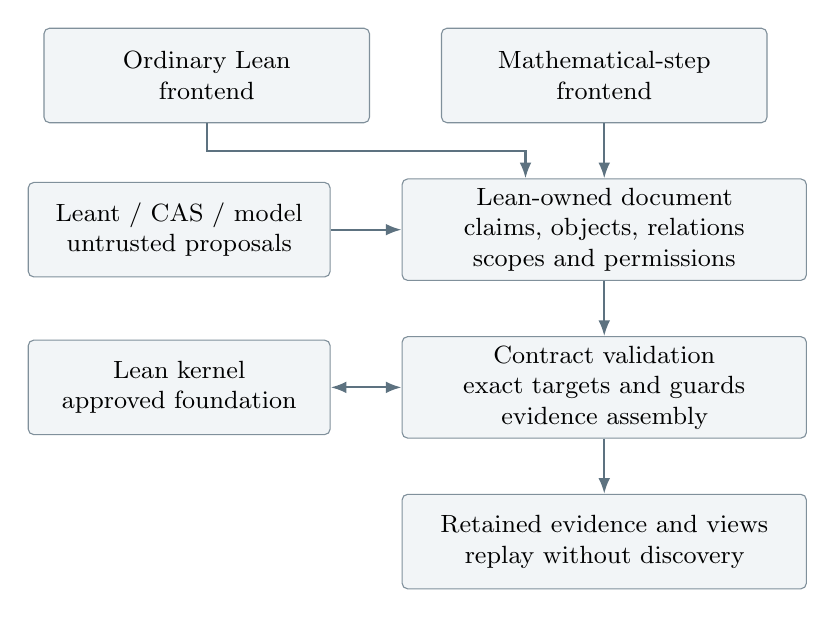
\begin{tikzpicture}[node distance=7mm and 9mm,
 box/.style={draw=ink!55,rounded corners=2pt,align=center,font=\small,
 fill=pale,minimum height=12mm,text width=39mm},
 arr/.style={-{Latex[length=2mm]},thick,draw=ink!70}]
\node[box] (lean) {Ordinary Lean\\frontend};
\node[box,right=of lean] (surface) {Mathematical-step\\frontend};
\node[box,below=of surface,text width=49mm] (core) {Lean-owned document\\claims, objects, relations\\scopes and permissions};
\node[box,left=of core,text width=36mm] (providers) {Leant / CAS / model\\untrusted proposals};
\node[box,below=of core,text width=49mm] (check) {Contract validation\\exact targets and guards\\evidence assembly};
\node[box,left=of check,text width=36mm] (kernel) {Lean kernel\\approved foundation};
\node[box,below=of check,text width=49mm] (artifact) {Retained evidence and views\\replay without discovery};
\draw[arr] (lean.south) -- ++(0,-3.5mm) -| ([xshift=-10mm]core.north);
\draw[arr] (surface) -- (core);
\draw[arr] (providers) -- (core);
\draw[arr] (core) -- (check);
\draw[{Latex[length=2mm]}-{Latex[length=2mm]},thick,draw=ink!70] (check) -- (kernel);
\draw[arr] (check) -- (artifact);
\end{tikzpicture}
\end{center}
The diagram separates responsibilities, not necessarily operating-system processes. Untrusted generated code needs process isolation in deployment. A private prototype can be smaller, but its accepted-evidence protocol should not depend on a shared mutable session being trustworthy.

\subsection{Methods: theorem first, policy second}
For a theorem-backed method, the logical contract is the instantiated theorem type. Roles identify author inputs, generated data, premises to attempt routinely, and premises that should be shown prominently. The latter two categories do not change the premise's logical status. The operational policy names allowed methods, normalization choices, budgets, and explanation templates.

A composite local-calculus theorem can package open-set membership, eventual equality, and derivative transfer. A normalizer additionally needs reification and a correctness theorem. An induction plan additionally needs a motive, recursor, and case coverage. These are three implementation families, not forty unrelated little languages.

All helper theorems and checker libraries must be available to the ordinary Lean frontend. Otherwise the evaluation would confuse a useful library abstraction with a useful new syntax.

\subsection{What Leant already contributes}
Leant's committed \path{Verification.hs} documents that its opaque \code{Verified} wrapper records callback acceptance, not a kernel proof, solver certificate, or behavioral theorem. It implements lazy, success-quota-aware verification of candidate groups and variants; the keyed verifier suppresses a spelling only after it was accepted~\cite{leantverification}. These are good scheduling and identity practices to retain, not evidence formats to overinterpret.

Its \path{Fragment.hs} decomposes supported structural forms and retains other forms as opaque atoms. The inspected source describes term-indexed applications as opaque and carries safety metadata for negative outcomes~\cite{leantfragment}. The adapter should preserve those capability reports while giving opaque atoms Lean-owned identities in the original environment.

The syntheses also review tactic suggestions, behavioral predicates, and working-tree extensions. Those observations concern their captured sources, including uncommitted changes, rather than necessarily this public commit~\cite{synthesis,blueprints}. They motivate requirements below; they are not fresh runtime findings of this article.

\subsection{The proposed request and response}
The adapter sends a reference to an immutable Lean request, a supported structural projection, and a bounded inventory of premises. It does not ask the Haskell engine to reconstruct the mathematical statement from a display string.
\begin{lstlisting}
Request:
  origin = (environment, document_revision, node, scope)
  telescope = ordered dependent binders
  target = exact Lean expression
  projection = structural view plus opaque expression handles
  permission = local facts, library inventory, axiom policy
  budget = total request limits and cancellation token

Response:
  CandidateTerm | CandidateEdit | CandidatePlan
  | Unsupported(location, feature)
  | Exhausted | Cancelled
  | NegativeCandidate(certificate, stated scope)
\end{lstlisting}
These are wire-level sketches, not a complete serializable ABI. A candidate is accepted only after decoding, exact-target checking, policy validation, and retention of the actual evidence. Successful verification of one rendered variant does not authorize another variant that looks equivalent.

For a proof hole, any permitted term of the frozen proposition may be enough. For a data hole, show meaningful alternatives until the object and its specification are accepted. Finite behavioral tests can help rank exploratory candidates. Publication of a universal behavior claim requires a proof of that universal claim; a collection of examples is not promoted to it.

\subsection{Negative outcomes need a different authority}
For a positive candidate, lossy search can still be useful: the candidate is checked at the original Lean target. For a negative result, the analogous shortcut is unavailable. The initial adapter should publish a refutation only when it has a Lean proof of the negated original proposition, or a certificate whose soundness and translation adequacy are both proved and composed into that proof.

A complete search over a restricted abstraction may establish that the abstraction has no solution. Its diagnostic should say exactly that, with the restriction and any budget qualification. A list of omitted nodes, however informative, is not a proof that nothing was omitted incorrectly. This avoids turning an engineering capability flag into an unstated axiom.

\subsection{Tactic edits, completion, and failures}
The exact proposed replacement text must be replayed from the same origin before it is called an accepted edit. A successful tactic's ``Try this'' message is a source of candidates; it is not a proof that the displayed text has the same behavior. The reports' discussion of \code{says} makes the distinction particularly clear: comparing a discovered suggestion with frozen text is not the same operation as executing that frozen text, and neither alone is a search-free term archive~\cite{synthesis,blueprints}.

The protocol separates progress, closure of a focused goal, completion of the entire root proof, and replay of the displayed edit. Whole-proof completion checks the root evidence, unresolved metavariables, admissions, exact target, and permitted dependency closure. A decline in visible goal count establishes none of those by itself.

Per-candidate heartbeats are not a total budget. The request budget covers generation, decoding, all failed variants, checking, and retained results. A worker generation and request origin prevent a late answer after undo from entering the current proof. Shared metavariables are committed transactionally. A speculative worker crash should lose that speculation, not corrupt the accepted document.

\section{Six worked mathematical cases}\label{sec:cases}
The examples below are mathematical derivations and interface specifications. The proposed source blocks are not compiled proofs. Their purpose is to make the promised abstraction accountable: each short command is followed by the mathematics, premises, and nearby failure that its implementation must handle.

\subsection{Binomial inversion without a hidden field hypothesis}\label{sec:binomialcase}
The inspected ProveIt module proves the integer kernel identity
\begin{equation}\label{eq:kernel}
 \sum_{k=j}^{n}(-1)^{n-k}\binom nk\binom kj
 =\begin{cases}1,&n=j,\\0,&n\ne j.\end{cases}
\end{equation}
An interval with $n<j$ is empty. In the other case, write $n=j+m$ and reindex by $k=j+i$, $0\leq i\leq m$. The binomial product identity gives
\[
 \binom{j+m}{j+i}\binom{j+i}{j}
 =\binom{j+m}{j}\binom mi.
\]
The left side of~\eqref{eq:kernel} therefore becomes
\[
 \binom{j+m}{j}\sum_{i=0}^{m}(-1)^{m-i}\binom mi.
\]
The inner sum is $(1-1)^m$: it is zero for $m>0$ and one for $m=0$, in which case the outer factor is also one. This proves the identity.

The source's cast normalization and interval conversions implement precisely this argument~\cite{binomial}. A useful method interface would let the author specify the substitution, the combinatorial identity, and the alternating row theorem:
\begin{lstlisting}
claim kernel_identity(n,j) : integer kernel sum = delta(n,j)
proof
  if n < j, conclude by empty interval
  otherwise write n = j + m
  reindex k := j + i with i in [0..m]
  rewrite the binomial product using choose_product
  calculate by integer polynomial algebra and alternating_row
\end{lstlisting}
The guard ledger contains coverage and inverse properties of $i\mapsto j+i$, the bounds needed for natural subtraction, the exact integer interpretation of the casts, and the branch condition $m=0$ or $m>0$. Some are discharged by arithmetic; the combinatorial identity remains a mathematical input.

For sequences in an additive commutative group $M$, let
\[
 b_n=\sum_{k=0}^{n}\binom nk\,\mathbin{\bullet}a_k,
\]
where the coefficients act by integer scalar multiplication. Substituting this into the proposed inverse and exchanging two finite sums leaves the coefficient in~\eqref{eq:kernel} on each $a_j$. The identity coefficient selects $a_n$ and annihilates the rest. No division, rational algebra, or multiplication of elements of $M$ is required.

This is a strong test of the CAS layer. It may normalize the \emph{integer coefficients} while treating the $a_j$ as module atoms. It may not make the proof easier by assuming $M$ is a field. A noninjective index map must fail the bijection method or switch, visibly, to a multiplicity-aware theorem. Omitting the upper endpoint fails the $n=j$ case; that case belongs in the package's negative-neighbor tests.

\subsection{Local differentiation and a reusable symbolic derivative family}\label{sec:odecase}
Assume $U\subseteq\R$ is open and
\[
 W'(x)=\varphi(W(x))\qquad(x\in U).
\]
Let $G_n$ have a derivative $H_n$ at the relevant values $W(x)$, with
\[
 G_0(W(x))=W(x),\qquad
 G_{n+1}(W(x))=H_n(W(x))\varphi(W(x)).
\]
Then
\begin{equation}\label{eq:ode}
 D^nW(x)=G_n(W(x))\qquad(n\in\N,\ x\in U).
\end{equation}
The induction must retain the whole assertion on $U$. At the successor step, fix $x\in U$. Openness gives a neighborhood on which the induction identity holds. Derivative congruence transfers the derivative of $D^nW$ to that of $G_n\circ W$. The chain rule supplies
\[
 (G_n\circ W)'(x)=H_n(W(x))\varphi(W(x))=G_{n+1}(W(x)).
\]
This proves the successor step. Notice that no global differentiability assumption on $G_n$ was used. Only the values in $W(U)$ matter, exactly as in the source theorem~\cite{ode}.

The shorter surface could be:
\begin{lstlisting}
induct n with invariant forall x in U, D[n] W(x) = G(n,W(x))
  zero: conclude using initial_family
  successor:
    fix x in U
    differentiate the induction identity locally at x on U
      using derivative_family and autonomous_equation
    conclude using family_recurrence
\end{lstlisting}
The word \code{locally} selects the eventual-equality contract. Replacing the hypothesis by equality at one point must fail this method: $f(t)=t$ and $g(t)=0$ agree at zero but have different derivatives there.

A useful hybrid specialization is $W'=W^2$. Let
\[
 G_n(w)=n!w^{n+1},\qquad H_n(w)=(n+1)!w^n.
\]
The ordinary power derivative gives $G_n'=H_n$, and polynomial arithmetic yields
\[
 H_n(w)w^2=(n+1)!w^{n+2}=G_{n+1}(w).
\]
Consequently $D^nW=n!W^{n+1}$ on $U$. The CAS performs symbolic derivative and polynomial normalization work; the proof assistant supplies the induction and local-analysis theorem. For arbitrary $n$, the certificate invokes a parameterized derivative theorem and factorial identity, not a finite table of computed derivatives.

This division of labor avoids two bad extremes: manually reproducing every local-calculus bridge, and allowing a CAS derivative command to infer unproved regularity or equality domains.

\subsection{Abel coefficients: a specification is not a chosen implementation}\label{sec:abelcase}
Let $A$ be a commutative $\Q$-algebra, let $a,x\in A$, and let $T\in A\llbracket t\rrbracket$ satisfy
\[
 T=t\exp(-aT).
\]
Here exponentials and substitution are \emph{formal} operations. The source derives the needed constant-coefficient and substitution facts from the functional equation, and proves the coefficient formula for any such $T$~\cite{abel}.

For $n\geq1$, the formal Lagrange--B\"urmann calculation is
\begin{align*}
 [t^n]\exp(xT)
 &=\frac1n[u^{n-1}]\,x\exp(xu)\exp(-nau)\\
 &=\frac{x}{n}[u^{n-1}]\exp((x-na)u)\\
 &=\frac{x(x-na)^{n-1}}{n!}.
\end{align*}
The rational factors in this display mean their images under the specified map $\Q\to A$. At $n=0$, the coefficient is one. The positive-index formula must not be extrapolated to zero by interpreting a negative exponent or dividing by zero.

A surface exposing exactly the mathematical argument is:
\begin{lstlisting}
fix T : FormalSeries A satisfying T = t * exp(-a*T)
have T_admissible by formal_implicit_series using its specification

for n >= 1:
  extract coefficient n of exp(x*T)
    by Lagrange_Burmann using T_admissible and its specification
  combine the formal exponentials
  calculate the coefficient by rational_scalar_algebra(A)

at n = 0:
  conclude by constant coefficient
\end{lstlisting}
The logical premises of the registered Lagrange theorem, rather than the English name, determine the real guard list. The source includes an inverse relation for the relevant formal series; a wrapper can derive it from $\exp(-au)\exp(au)=1$ and the admissible substitution. It cannot assume that every arbitrary expression passed to \code{subst} is automatically admissible.

The scalar calculation must remain valid even when $A$ has zero divisors. A nonzero rational has an inverse in $\Q$, and its inverse identities map into $A$. Thus the image of the positive integer $n$ has a specified inverse sufficient for cancellation. This argument does not require $A$ to be a field or the algebra map to reflect equality. In the trivial ring all the mapped identities still hold; a gratuitous nontriviality assumption would weaken the source theorem.

The definition package can also expose a canonical Abel series constructed by compositional inversion. That construction is useful computationally, but the coefficient theorem above is not allowed to replace the arbitrary $T$ by it merely because that makes computation convenient. A uniqueness theorem could justify such a replacement; otherwise the arbitrary specification remains the theorem's interface.

Finally, extracting the first hundred coefficients gives a hundred exact facts or one finite-precision fact. It is not the displayed formula for all $n$. Moving from the formal identity to an equality of analytic functions similarly requires convergence and compatibility theorems. These are two independent boundaries: finite versus universal, and formal versus analytic.

\subsection{Natural arithmetic: retain the guards or change the proof visibly}\label{sec:sqrtcase}
Write $s=\lfloor\sqrt n\rfloor$ and
\[
 S=\sum_{k=1}^{n}\lfloor\sqrt k\rfloor.
\]
The ProveIt theorem states a natural-number equality
\[
 S=s(n+1)-\frac{s(s+1)(2s+1)}6.
\]
The subtraction and division on the right are natural operations. The inspected proof explicitly establishes the conditions permitting transport to its rational companion~\cite{sqrt}.

There is a useful alternative argument, already proposed in the first-round reports and discussed by both syntheses, so not claimed here as a new mathematical discovery~\cite{synthesis,blueprints}. Count pairs $(j,k)$ with $1\leq k\leq n$ and $1\leq j\leq\lfloor\sqrt k\rfloor$. Counting first by $k$ gives $S$. Counting by $j$ gives
\[
 S=\sum_{j=1}^{s}(n+1-j^2).
\]
Since $j\leq s$ implies $j^2\leq n$, there is no negative cardinality. It follows in the naturals that
\[
 S+Q=s(n+1),\qquad Q=\sum_{j=1}^{s}j^2,
 \qquad 6Q=s(s+1)(2s+1).
\]
The last identity is the standard finite sum-of-squares polynomial identity and can be proved by induction and ring normalization. Together these equations establish both the division certificate and the subtraction bound. Consequently the displayed natural closed form equals $S$.

This illustrates a useful preference: \emph{avoid a lossy representation operation when the mathematics supplies a balance equation}. The language may propose the counting proof as a plan change, not pretend that it merely optimized the original rational-induction proof.

Whether the author keeps the original proof or adopts the counting argument, the CAS should receive exact algebraic obligations and return the same natural theorem. Nearby failures are $(2-3:\N)$ transported as $2-3$ in $\Z$, and $(3/2:\N)$ transported as $3/2$ in $\Q$. Both are false bridges, not merely missing hints.

\subsection{An exact algebraic root and a certified enclosure}\label{sec:rootcase}
Return to $p(x)=x^3-x-1$. We now spell out the certificates behind Section~\ref{sec:session}.

At the endpoints of $[1,2]$, $p(1)=-1$ and $p(2)=5$. Polynomial evaluation defines a continuous real function. The intermediate value theorem therefore gives a root in $(1,2)$. Also
\begin{equation}\label{eq:derivcert}
 p'(x)=3x^2-1=2+3(x-1)(x+1)\geq2
 \qquad(1\leq x\leq2).
\end{equation}
For $u<v$ in this interval, the mean value theorem gives
$p(v)-p(u)\geq2(v-u)>0$. Hence the root in $[1,2]$ is unique.

The exact rational endpoint calculations are
\[
 p\!\left(\frac{331}{250}\right)=-\frac{47809}{15625000}<0,
 \qquad
 p\!\left(\frac{53}{40}\right)=\frac{77}{64000}>0.
\]
Both rational endpoints lie strictly between one and two. By continuity there is a root between them, and uniqueness identifies it with the already accepted root $r$. Therefore
\begin{equation}\label{eq:rootbound}
 \frac{331}{250}<r<\frac{53}{40}.
\end{equation}
The interval width is $1/1000$. Its midpoint $2649/2000$ is a numerical approximation satisfying
\[
 \left|r-\frac{2649}{2000}\right|<\frac1{2000}.
\]
It is not an exact expression for $r$.

The computational certificate consists of the two rational signs and the polynomial derivative identity~\eqref{eq:derivcert}. The real-analysis contract contributes continuity, existence, and uniqueness. The software need not ask the CAS to emit a proof of the intermediate value theorem. It must apply the already proved theorem with the correctly checked data.

This contract asserts uniqueness in $[1,2]$, which is all the session requested. A claim about all real or complex roots would be a different target with additional obligations. Replacing the interval by one containing no root, or replacing a strict endpoint sign by zero, changes the method's applicability. A correct alternative bracketing theorem may handle endpoint roots, but that change must be explicit.

\subsection{Radical denesting and branch-aware checking}\label{sec:radicals}
A hybrid CAS should be useful for exploratory radical denesting without confusing a candidate formula with a theorem. For example, a producer suggests
\[
 \sqrt{3+2\sqrt2}=1+\sqrt2.
\]
A small real-algebra contract can check this by establishing $\sqrt2\geq0$, $(\sqrt2)^2=2$, $1+\sqrt2\geq0$, and
\[
 (1+\sqrt2)^2=3+2\sqrt2.
\]
Uniqueness of the nonnegative square root then proves the identity. The producer could be an unverified denesting algorithm; the verification theorem uses only its candidate and exact evidence.

The negative candidate $-1-\sqrt2$ satisfies the same squared equation but fails the nonnegative-branch condition. This is why ``square both sides and normalize'' is not a complete denesting checker. For complex radicals, a real sign condition must be replaced by the actual branch convention and relevant argument-domain theorems. No generic real checker should quietly switch to complex principal roots.

A method can be progressively generalized. Initially accept towers of real square roots with explicit radicand and sign evidence. Next add an algebraic-number representation with root isolation and equality checking. Only later consider a completeness theorem for a particular denesting class. ``No candidate found'' remains a search outcome until that much stronger theorem and its decision procedure exist.

This use case captures the intended hybrid: a CAS proposes compact mathematical objects, theorem-backed checks establish their exact meaning, and the accepted object becomes available for subsequent symbolic calculations and proofs.

\section{Publication, explanations, and maintenance}\label{sec:publication}
\subsection{A mathematical document, not just its final theorem}
Every formal assertion in the source must have accepted evidence, including an unused intermediate assertion. A proof of the final theorem by an unrelated shortcut does not validate a false sentence earlier in the document. True unused claims can remain, visibly marked as unused. Informal commentary is allowed but must be distinguished from checked assertions.

The typed document supports three synchronized views: a mathematical argument, an obligation view, and detailed evidence. A small additional panel records semantic choices: the domain, branch, coefficient structure, interpretation of subtraction and division, selected representative, and approximation relation. It need not display every kernel argument to be useful.

A named computational step should show its actual contract. For example, ``rational normalization under $x\ne1$'' is generated from the accepted method and guard. It should not be replaced by a persuasive model-generated sentence about continuity if the step used no continuity argument. Method conformance certifies the designated construction of the proof, not that the reason was logically indispensable or that it matches a human's private reasoning.

An author may request an unrestricted checkpoint proof. Its display says that the claim was established by permitted automation, with the actual evidence expandable. It must not pretend to implement a more specific plan that the source did not require.

\subsection{Visibility should follow mathematical importance}
Default display collapses routine proofs of already apparent bounds and scalar identities. It keeps substantial analytic premises, new branch choices, changed domains, and nontrivial representation changes visible. A user who expands a guard sees its exact proposition, how it was discharged, and the assumptions used.

Notices about total division or formal-series interpretation have a different status from open obligations. Notices disclose meaning; they are not failed proofs. A dismissal can be recorded for a specific occurrence or for an explicit project convention, tied to the relevant resolved meaning. Changing that meaning invalidates the dismissal. A project-wide setting should not suppress a newly introduced branch convention merely because it once suppressed a harmless total-division notice.

The renderer should support a defined round-trip subset and semantic difference tests. Deterministic output is not automatically faithful output. Reader experiments must test whether users can distinguish changed quantifier dependence, domains, and precision from the displayed text.

\subsection{The publication artifact}
An accepted document should export the controlled source or Lean source, expanded readable Lean, retained term-level evidence or checked certificate payloads, a statement-and-environment manifest, a source map, a dependency and axiom audit, and method/checker identities. The proof terms and exact target in the pinned environment are authoritative for proof validity; the readable source remains an essential review artifact.

Publication rechecks the final terms at their exact targets and checks coverage of the source assertions. A transitive allowlist applies to the actual axiom inventory, not just a textual search for a historically named admission constant. Reference-algorithm evaluation and certificate checking obey the same computation policy. Policies permitting extra computation assumptions can exist, but their artifacts carry a different assurance label.

Search-free replay means no invocation of Leant, a model, a remote CAS, or heuristic theorem discovery. It can still include deterministic checking computation. Replaying a tactic script that runs a search procedure is not this mode, even when its source text is frozen. A retained certificate whose verified checker computes deterministically is acceptable under the declared checking policy.

\subsection{Two representations do not create two authorities}
A proof term and a readable script can diverge after an upgrade. The system must then report a mismatch or migration requirement. It must not choose whichever version succeeds and describe that as unchanged replay. Old evidence remains interpretable relative to its old pinned environment; a new environment requires rechecking and a new artifact.

Classify edits into the four categories already proposed by the first synthesis: evidence-only, plan, object, and statement~\cite{synthesis}. Only evidence-only changes are eligible for automatic replacement under an existing policy. A plan can change the induction motive or decomposition without changing the theorem. An object change can select another witness. A statement change can alter a domain or hypothesis. All three require an explicit mathematical diff.

Hashes identify artifacts and detect mismatches; they do not establish mathematical truth. A certificate package needs actual content and a validating interpretation. An imported binary environment also has an operational validation boundary. For unreviewed generated code, the checking process should be isolated from discovery and tied to a separately fixed target; these precautions align with Lean's validation guidance~\cite{validation}.

\subsection{Cost and comprehensibility are not secondary}
Proof-producing computation can generate enormous terms. A production design should share repeated subcertificates, retain DAG structure where supported, cache checks by validated dependencies, and prefer compact certificates over long tactic traces. Cache validity includes definitions and structures used by a calculation, not only the target's printed string.

The service reports generation time, checking time, certificate size, and replay work separately. A one-line calculation that regularly spends minutes elaborating hidden proof terms may be worse than a slightly longer explicit proof. Likewise, a perfectly checked document whose central analytic premise is hidden by default can fail its explanatory purpose. These are design failures even when logical soundness is preserved.

\section{Executable evidence and an evaluation that can reject the proposal}\label{sec:experiment}
\subsection{What was executed for this article}
The archive includes \path{certificate_demo.py}, a standard-library Python reference experiment using exact \code{Fraction} arithmetic. It models a narrow boundary: a caller-owned rational-function identity, a proposed polynomial cross-product certificate, and the denominator guards that remain attached to an accepted conditional result.

The checker recomputes the polynomial identity and expected guard list. It rejects a different request origin, an altered target, a stale revision, a different scope, a forged residual polynomial, and omitted or changed denominator guards. An identically zero denominator is explicitly unsupported by this particular contract; that rejection does not mean every equality involving total division by zero is false. The program never accepts a provider-supplied ``proved'' flag.

The test run completed with \textbf{25 tests passed, zero failures, and zero errors}. One test contains 182 finite binomial-orthogonality instances. Other tests verify the exact rational endpoint values in~\eqref{eq:rootbound}, the polynomial identity in~\eqref{eq:derivcert}, the counterexample to unguarded cancellation, and the loss of one coefficient order under differentiation. The machine-readable record is \path{experiment-results.json}.

These are tests of a small Python model, not a formal proof of its implementation and not a test of Lean, Leant, a frontend, or a compiler. In particular, the Python program does not verify the intermediate value theorem, prove the correctness of \code{Fraction}, implement a dependent telescope, or establish the binomial identity for all indices. The general mathematical arguments are given in this article; formalization remains implementation work.

The experiment is included because it gives the next iteration something concrete to replace: port the request boundary, polynomial checker, and its guard discipline to Lean; prove soundness there; then retain the same nearby-invalid cases as regression tests.

\subsection{Separate the effects being measured}
A comparative study needs at least three configurations:
\begin{enumerate}
\item Existing idiomatic Lean, with reasonable expert refactoring.
\item Ordinary Lean with the same new definition packages, computation services, theorem wrappers, and Leant access proposed here.
\item The \Noema\ frontend with exactly that shared infrastructure.
\end{enumerate}
The second-minus-first comparison measures the shared library and automation package. The third-minus-second comparison measures the new surface and document interaction. A further rendered-view treatment can test whether the benefits require new authored syntax at all.

Tasks should include a stratified compiled sample from the four inspected source families, nearby variants, and a held-out family. Split by theorem or module before harvesting subgoals. Exclude the target theorem, downstream consequences, aliases, retained answers, and revealing caches from providers' permitted dependency closure. The complete allowed environment should be recorded. A held-out theorem is not held out if its answer is available under another name.

\subsection{What to measure}
Record authoring and repair time, explicit mathematical choices, failed attempts, unresolved guards, median and tail latency, total checking work, certificate size, and dependency churn. For readers, ask for the key idea, the hypothesis enabling a step, the effect of changing a bound, and the location of a deliberately invalid move. Prior Lean and mathematical experience are relevant covariates.

Source length is descriptive, not the objective. A helper theorem tailored to a single example can make any language appear concise. Charge the creation and maintenance of helpers, method wrappers, checkers, and definition packages. Report the infrastructure cost separately and its observed reuse over held-out tasks, rather than amortizing it over imagined future proofs.

Useful ablations remove the new syntax, verified CAS service, definition package, contextual guard index, broad retrieval, or strict method conformance one at a time. If removing the syntax preserves the gains, keep the library and document view. If removing the CAS destroys the gains in both frontends, credit the computation service rather than the language.

\subsection{A contract-level adversarial suite}
\begin{longtable}{@{}P{.36\textwidth}P{.56\textwidth}@{}}
\toprule
Mutation & Required response \\
\midrule\endhead
Delete $x\ne1$ from cancellation & Retain the conditional result or leave the guard open; do not publish the global equality.\\
Replace a neighborhood identity by a point identity & Refuse derivative transfer and identify the missing locality premise.\\
Differentiate an order-$N$ jet without extra input precision & Produce order $N-1$ when justified, or request more precision for the unchanged target.\\
Use finitely many coefficients for a universal identity & Retain only the finite statement; require a uniform proof.\\
Interpret formal substitution analytically & Require a separate convergence and interpretation theorem.\\
Transport natural subtraction or division without guards & Expose nontruncation or exact-division obligations.\\
Replace an additive group by a field & Treat as a changed theorem, never as a proof improvement.\\
Replace arbitrary Abel $T$ by the canonical series & Require proved equality/uniqueness and explicit transport, or keep the original object.\\
Accept the negative square-root branch & Reject the branch specification even if the squared identity holds.\\
Call one isolated root a complete solution set & Require a completeness theorem and root-enumeration evidence.\\
Reuse a certificate in a sibling branch or after undo & Reject the origin and scope mismatch.\\
Use a result to prove its own guard & Reject cyclic or ill-scoped proof assembly.\\
Add a nonreflecting representation route & Refuse the return implication; preserve the previously pinned route.\\
Infer refutation from provider exhaustion & Report exhaustion, not a negative theorem.\\
Display an unreplayed tactic replacement & Label it a proposal until the exact edit is checked at its origin.\\
Hide a false unused assertion behind a valid final proof & Reject publication of the document.\\
Admit unapproved computation axioms transitively & Fail the publication policy even if the declaration typechecks.\\
Change the meaning while retaining printed notation & Invalidate the relevant seal and show an object/statement diff.\\
\bottomrule
\end{longtable}
These tests specify \emph{which conclusion must not be accepted}, not that every mutated theorem is false. A different valid method may prove some neighbors. Conversely, a service that rejects every positive example is safe but useless; each negative test therefore needs a positive companion and an expected diagnostic location.

\subsection{Go/no-go decisions}
Correctness gates are nonnegotiable: no target weakening, no silent object replacement, no scope escape, no false all-assertion acceptance, and no policy bypass. Usability thresholds should be set after a pilot reveals realistic variance, not invented here as authoritative percentages.

The project should explicitly allow three successful outcomes: a new authored language, a rendered mathematical document layer, or a Lean library plus tooling. The last outcome is not failure if it removes actual work. The design should be abandoned or narrowed if the shared services cost more to maintain than they save, or if the surface makes readers systematically miss essential premises.

\section{Implementation sequence and remaining research}\label{sec:roadmap}
\subsection{First slice: one real calculation, end to end}
Begin with a Lean-owned claim record, an explicit theorem wrapper, exact target retention, a guard ledger, and accepted proof evidence. Expose it through both ordinary Lean and a minimal mathematical-step block. Implement polynomial identity checking and guarded rational cancellation using the existing library where possible, with a clearly specified strict checking path.

The completion criterion is not that the demonstration reads well. It is that the identical target is checked, the omitted-guard neighbor is not accepted, the exact evidence can be replayed with the producer disabled, and an edit changing the denominator invalidates the right evidence. This single slice exercises most of the architecture without a large language implementation.

\subsection{Second slice: the two nontrivial ProveIt bridges}
Add finite reindexing and local derivative transfer. The first tests binders, membership facts, natural subtraction, and finite-support reasoning. The second tests a relation other than equality, an open-set-to-neighborhood bridge, and preservation of range-local hypotheses.

Use ordinary wrapper theorems shared by both frontends. Demonstrate the integer kernel proof and the autonomous derivative theorem, then test held-out neighboring files before adding more surface features. Do not use the final target theorem as a helper or compare against a deliberately unrefactored baseline.

\subsection{Third slice: definitions and precision}
Package the Abel series interface, keeping arbitrary specifications separate from canonical construction. Add exact finite-series arithmetic with a proved coefficient-agreement contract and differentiation's precision shift. Measure how many obligations are removed by the package itself, separately from any gain in syntax.

This is where the CAS becomes more than a collection of tactics: it works with durable objects, retains multiple representations of them, and plans computation from the observations a proof requests. It also tests the strongest new design claim in this article, namely that managing a computation's relation and precision at the language level can prevent errors that a tactic-name wrapper does not address.

\subsection{Fourth slice: Leant and data construction}
Measure Leant's value on structural \emph{compositions}, separately from single-lemma applications already accessible to ordinary retrieval. Connect its existing engine through the exact-origin adapter rather than rewriting the engine first. Add the root-specification and enclosure session, with separate proof of existence and construction of a computational representation.

The two frontends should now share the same immutable requests, method/checker library, candidate policy, and evidence format. Only after this point should natural-language drafting and proof-lifting be expanded. Lifting existing Lean must preserve the resolved declaration and retain unrecognized fragments as Lean blocks; guessing a false high-level reason is worse than leaving a low-level block visible.

\subsection{What remains difficult}
Three technical problems deserve focused research. The first is efficient reification and proof reconstruction for symbolic expressions with binders and dependent parameters. The second is predictable composition of representations, particularly where precision or an accepted data object changes. The third is proof compression that preserves source-to-evidence correspondence without creating expensive or opaque checking work.

Three usability problems are equally important: choosing default visibility for guards, making statement differences legible, and discovering which methods a mathematician can invoke without knowing the library's implementation details. Role metadata, contextual indexing, and aliases can help, but their benefit is an empirical hypothesis.

No general theorem here proves semantic fidelity of the frontend or correctness of its compiler. Relative proof soundness has the familiar conditional form: if the fixed targets and scopes are correctly retained, every generated obligation has checked evidence, the dependent assembly is well typed, and the final terms are rechecked under the policy, then the accepted claims have proofs. That is a useful invariant, not a substitute for implementing and testing the boundary. The finite-precision and worked-case propositions in this article are mathematical proofs, not a completed mechanized metatheory.

\clearpage
\section{Conclusion}
The best second-round proposal is not another vocabulary for ``have, then, therefore.'' The syntheses already converge on the right conservative foundation. The missing opportunity is to let a mathematician \emph{calculate with formally specified objects} without surrendering control of domains, branches, precision, or generality.

\Noema\ would make a computation's exact relation part of its interface, retain the guards under which it is valid, and connect mathematical definitions to computational representations through proved packages. Its CAS core would be built from verified algorithms and verified checkers, with optional untrusted acceleration. Leant would supply structural candidate generation under the same exact-target acceptance boundary. The author writes the mathematical choices; the system reconstructs their consequences and preserves the evidence.

The immediate recommendation is modest: build the shared Lean-owned calculation protocol, polynomial and guarded-rational services, finite reindexing, and local derivative transfer. Then test definition packages and precision-aware computation on the Abel development. The authored language should earn its place against ordinary Lean with the same infrastructure. A successful result may be a new language, or it may be a much better way to write, compute, read, and maintain mathematics in Lean.

\clearpage
\appendix
\section{Answers to the syntheses' next-round questions}\label{app:answers}
The decisions below answer the two reports' question sets rather than pose another unprioritized agenda. The question labels are local to this appendix; the wording abbreviates the original questions~\cite{synthesis,blueprints}.

\subsection{The ten questions in \emph{Mathematical Ideas, Checked Evidence}}
\begingroup\small
\begin{longtable}{@{}P{.34\textwidth}P{.58\textwidth}@{}}
\toprule
Question & Decision in this proposal \\
\midrule\endhead
S1. What is the smallest useful step contract? & Use an ordinary wrapper theorem for logical methods; add explicit reification/checker contracts for computations and recursor contracts for structural plans. Do not force all three into an attribute alone.\\
S2. Is a stated reason binding? & A named transformation is method-constrained. An explicit open proof request is not. The accepted method node, rather than an informal explanation, records conformance.\\
S3. Which choices may automation make? & Proof evidence and approved representation housekeeping can be automatic. Plan changes, retained-object changes, and statement changes are proposed as distinct reviewable edits.\\
S4. What does an accepted suggestion guarantee? & The exact displayed edit has been checked from its recorded origin; root completion and axiom-policy acceptance have their own statuses. A successful probe of different text is insufficient.\\
S5. How should infrastructure cost be counted? & Compare equally equipped Lean and the new frontend. Report implementation and maintenance cost of each method/checker/package separately, with observed reuse rather than assumed amortization.\\
S6. How do multiple views compose? & Compose their actual dependent contracts in order. Pin routes initially; allow automatic alternatives only with registered coherence evidence at the required observation and domain.\\
S7. What protects statement fidelity? & Resolve and retain meaning, render semantic choices, distinguish notices from obligations, and review object/statement differences. Do not claim that a deterministic printer proves human intent.\\
S8. What survives replay and upgrades? & Retained terms/certificates in a pinned environment are the checking authority; readable source is retained too. An upgrade creates a rechecked artifact, not silent cross-version replay.\\
S9. How do definitions and observational replacement enter? & Start with specification templates and pinned representatives. Observation-relative replacement is permitted only where all affected uses have explicit congruence/transport evidence.\\
S10. What belongs in the published view? & Every checked assertion, its status, essential hypotheses and choices, plus expandable guards and evidence. Rejected alternatives are optional provenance, not part of mathematical validity.\\
\bottomrule
\end{longtable}
\endgroup

\clearpage
\subsection{The twelve questions in \emph{Nine Blueprints}}
\begingroup\small
\begin{longtable}{@{}P{.34\textwidth}P{.58\textwidth}@{}}
\toprule
Question & Decision in this proposal \\
\midrule\endhead
B1. Document view or input language? & Support both on one typed document. Keep Lean first-class. Ship only the view when new syntax adds no measured value.\\
B2. How much is genuinely routine? & Instrument actual attempts and replay the selected portfolio on harvested goals. Lexical tactic counts alone cannot answer this.\\
B3. Where does analysis plumbing belong? & A small family of composite theorem wrappers plus local-equality relations. Wrap existing tactics only where procedural behavior is genuinely needed.\\
B4. Do method roles survive refactoring? & Put stable role IDs on project-local wrappers; validate them against the wrapper telescope. A binder-name mismatch fails migration instead of triggering inference by position.\\
B5. How are notices dismissed? & Per occurrence or explicit semantic convention, with the resolved meaning recorded. Invalidate affected dismissals when definitions, notation, or structures change.\\
B6. What is the unit of replay? & Retained checked terms and deterministic certificate-checking data, grouped by dependency. Tactic text is a readable/rebuild companion, not the sole evidence.\\
B7. Should every provider share Leant's outcome shape? & Share typed candidate and failure outcomes, but keep abstraction metadata separate from mathematical negative evidence. Refutation requires an original-target proof or proved adequacy plus a checked certificate.\\
B8. Is the structural adapter worth building? & Measure compositions separately from single theorem retrieval. Retain an adapter only where it improves the shared infrastructure under controlled budgets.\\
B9. What happens to data alternatives? & Show alternatives during discovery; pin the accepted object and prove its specification for publication. Retain rejected alternatives only as optional provenance.\\
B10. Where should definitions start? & Three narrow templates: finite indexed families, formal series, and uniquely specified algebraic objects. Compare their ordinary Lean APIs against the proposed surface.\\
B11. Who owns contracts and conflicting policies? & Versioned packages with explicit owners; qualify conflicting meanings; record composed search policies. No silent import-order override of mathematical interpretation.\\
B12. What is the stopping rule? & A library, linter, and document renderer are valid outcomes. Narrow or stop the language project if syntax brings no additional comprehension or authoring benefit.\\
\bottomrule
\end{longtable}
\endgroup

\Needspace{30\baselineskip}
\section{A minimal grammar and acceptance obligations}\label{app:grammar}
This grammar sketches the initial controlled surface. \code{Term} and \code{Prop} refer to resolved Lean syntax in a declared notation profile. It is not a complete parser specification.
\begin{lstlisting}
Document    ::= Declaration*
Declaration ::= LeanDeclaration | ObjectDecl | ClaimDecl
ObjectDecl  ::= "define" Name ":" Term ":=" Term
              | "construct" Name ":" Term "satisfying" Prop Method
              | "noncomputable select" Pattern "from" Term Method
ClaimDecl   ::= "claim" Name ":" Prop "proof" Block
Block       ::= Step*
Step        ::= "have" Name ":" Prop Method
              | "show" Prop Method
              | "calculate" RelationClaim Method
              | "obtain" Pattern "from" Term
              | "cases" Term CaseBlock
              | "induct" Term ["with invariant" Prop] CaseBlock
              | "suffices" Prop "via" Term Block
              | "lean" LeanBlock
RelationClaim ::= Term "=" Term
                | Term "=" Term "on" Term
                | Term "==" Term "mod" Term
                | "enclose" Term "in" Term
Method      ::= "by" MethodName ["using" Terms] [Policy]
              | "by open_proof" Policy
\end{lstlisting}
Surface convenience forms in the main text desugar into these nodes plus registered methods. The operational specification must state how binders and references are resolved; an English-looking phrase is not sufficient semantics.

A proof node is accepted only at its original proposition. A construction node is accepted with a value and its specification proof. A relation node is accepted at its declared relation, with every required guard proved or explicitly retained in a conditional result. An unresolved guard cannot be hidden inside an unconditional accepted node. A completed document checks every formal assertion and its scope, not just the final declaration.

An implementation should export a machine-readable schema for these requirements before adding many surface synonyms. The schema is the interchange format for ordinary Lean, the mathematical frontend, Leant, CAS providers, and benchmarks. It is also the unit that a future formally verified elaborator could target.

\section{Source register and reproducibility}\label{app:sources}
\subsection{Repository revisions and inspection scope}
The source review was static. The two requested synthesis reports were read closely, including their revised discussions and next-round questions. The four ProveIt modules below and the indicated Leant modules were inspected directly. The original nine proposals were considered through the two syntheses; they were not each reread in full for this article.

\begin{description}[style=nextline]
\item[Brainstorm]
\path{494be9d5ab41a5ae219fc6f800e6aee3c93bce39}. Both requested report sources. Their own reviewed local snapshots and historical audits retain their separate provenance.
\Needspace{6\baselineskip}
\item[ProveIt]
\path{24ce8bd743eaab64a91ce90725ea00f498d319d2}. Public source inspection of the four listed modules. The syntheses also refer to a different local revision:\par
\path{7c4e3f109405b9805b35d27ae96bf09c7ee5f3d5}.\par
This article does not equate the two snapshots.
\Needspace{6\baselineskip}
\item[Leant]
\path{3a40904be8a410d832d9ab6900b3d3e7b425eccb}. Direct inspection of \path{src/Leant/Synth/Verification.hs}, lines 1--210, and \path{src/Leant/Synth/Fragment.hs}, lines 1--140. The reports' modified working-tree suggestion and behavioral-synthesis review is attributed to them, not represented as a build of this public commit.
\Needspace{6\baselineskip}
\item[Mathlib availability check]
\path{Mathlib/Tactic/Polyrith.lean}, moving \code{master}, retrieved 5 September 2026 Pacific; returned Git blob \path{267384428fb20711dad86d0ff8be9f27b2c614a3}. This records the current-source observation, not a dependency chosen for a prototype.
\end{description}
The referenced external documentation was consulted on 5 September 2026 Pacific. Moving documentation is a source for architecture and availability checks, not a replacement for the toolchain pin of a future implementation. UTC timestamps on some retrieved repository commits fall on 6 September; that is still 5 September in Pacific time.

\subsection{Files in the accompanying archive}
\begin{tabularx}{\textwidth}{@{}P{.34\textwidth}Y@{}}
\toprule
File & Purpose \\
\midrule
\path{noema.tex} & Self-contained LaTeX source with embedded bibliography.\\
\path{noema.pdf} & Compiled article.\\
\path{certificate_demo.py} & Exact-arithmetic reference experiment; not a formally verified implementation.\\
\path{experiment-results.json} & Executed test counts, exact endpoint values, Python version, and program digest.\\
\path{source-register.json} & Repository/file identifiers and review scope.\\
\path{README.md}, \path{build.sh} & Status, contents, and reproducible build/run instructions.\\
\bottomrule
\end{tabularx}
The experiment can be rerun with
\begin{lstlisting}
python3 certificate_demo.py --output experiment-results.json
\end{lstlisting}
The article can be built using \code{latexmk -pdf noema.tex}. Its bibliography is embedded; no external bibliography database, network access, or supplied font files are needed. This archive does not contain an installed language, a compiled Lean project, or a claimed formal verification of the Python program.

\phantomsection\addcontentsline{toc}{section}{References}
\begin{thebibliography}{99}
\small
\bibitem{synthesis}
Codex. \emph{Mathematical Ideas, Checked Evidence: A Unified Evaluation of Nine Proof-Language Proposals}. Brainstorm, revised source, 5 September 2026.
\path{docs/synthesis/unified-report.tex}.
\href{https://github.com/VladimirReshetnikov/Brainstorm/blob/494be9d5ab41a5ae219fc6f800e6aee3c93bce39/docs/synthesis/unified-report.tex}{Pinned source}.

\bibitem{blueprints}
Claude (Anthropic). \emph{Nine Blueprints for a Mathematician's Proof Language over Lean}. Brainstorm, revised source, 5 September 2026.
\path{docs/unified_report/unified_report.tex}.
\href{https://github.com/VladimirReshetnikov/Brainstorm/blob/494be9d5ab41a5ae219fc6f800e6aee3c93bce39/docs/unified_report/unified_report.tex}{Pinned source}.

\bibitem{binomial}
Vladimir Reshetnikov and contributors. ProveIt, \path{Analysis/FabiusFunction/Lean/FabiusFunction/BinomialInversion.lean}.
\href{https://github.com/VladimirReshetnikov/ProveIt/blob/24ce8bd743eaab64a91ce90725ea00f498d319d2/Analysis/FabiusFunction/Lean/FabiusFunction/BinomialInversion.lean}{Pinned source}.

\bibitem{ode}
Vladimir Reshetnikov and contributors. ProveIt, \path{Analysis/FabiusFunction/Lean/FabiusFunction/AutonomousIteratedDeriv.lean}.
\href{https://github.com/VladimirReshetnikov/ProveIt/blob/24ce8bd743eaab64a91ce90725ea00f498d319d2/Analysis/FabiusFunction/Lean/FabiusFunction/AutonomousIteratedDeriv.lean}{Pinned source}.

\bibitem{abel}
Vladimir Reshetnikov and contributors. ProveIt, \path{Analysis/FabiusFunction/Lean/FabiusFunction/AbelPolynomialSeries.lean}.
\href{https://github.com/VladimirReshetnikov/ProveIt/blob/24ce8bd743eaab64a91ce90725ea00f498d319d2/Analysis/FabiusFunction/Lean/FabiusFunction/AbelPolynomialSeries.lean}{Pinned source}.

\bibitem{sqrt}
Vladimir Reshetnikov and contributors. ProveIt, \path{NumberTheory/IntegerSums/Lean/IntegerSums/FloorSqrtSum.lean}.
\href{https://github.com/VladimirReshetnikov/ProveIt/blob/24ce8bd743eaab64a91ce90725ea00f498d319d2/NumberTheory/IntegerSums/Lean/IntegerSums/FloorSqrtSum.lean}{Pinned source}.

\bibitem{leantverification}
Vladimir Reshetnikov and contributors. Leant, \path{src/Leant/Synth/Verification.hs}, especially callback receipts and candidate-group verification.
\href{https://github.com/VladimirReshetnikov/Leant/blob/3a40904be8a410d832d9ab6900b3d3e7b425eccb/src/Leant/Synth/Verification.hs}{Pinned source}.

\bibitem{leantfragment}
Vladimir Reshetnikov and contributors. Leant, \path{src/Leant/Synth/Fragment.hs}, especially the structural translation and opaque-atom boundaries.
\href{https://github.com/VladimirReshetnikov/Leant/blob/3a40904be8a410d832d9ab6900b3d3e7b425eccb/src/Leant/Synth/Fragment.hs}{Pinned source}.

\bibitem{validation}
The Lean development team. \emph{Validating a Lean Proof}. Lean Language Reference. Consulted 5 September 2026.
\url{https://lean-lang.org/doc/reference/latest/ValidatingProofs/}.

\bibitem{native}
The Lean development team. \emph{Lean.Meta.Native}: infrastructure for proofs by native evaluation. API documentation. Consulted 5 September 2026.
\url{https://lean-lang.org/doc/api/Lean/Meta/Native.html}.

\bibitem{harrison}
John Harrison and Laurent Th\'ery. A skeptic's approach to combining HOL and Maple. \emph{Journal of Automated Reasoning} 21, 279--294, 1998.
\href{https://www.cl.cam.ac.uk/~jrh13/papers/cas.html}{Author's paper page}; DOI: \href{https://doi.org/10.1023/A:1006023127567}{10.1023/A:1006023127567}.

\bibitem{lewiswu}
Robert Y. Lewis and Minchao Wu. A bi-directional extensible interface between Lean and Mathematica. \emph{Journal of Automated Reasoning} 66, 215--238, 2022. Preprint arXiv:2101.07758.
\url{https://arxiv.org/abs/2101.07758}.

\bibitem{interval}
Guillaume Melquiond and contributors. \emph{Interval Package for Rocq}. Documentation of interval, integral, root, and enclosure tactics. Consulted 5 September 2026.
\url{https://coqinterval.gitlabpages.inria.fr/}.

\bibitem{polyrith}
Mathlib contributors. \emph{Mathlib.Tactic.Polyrith}. Current-source availability notice, consulted 5 September 2026. Git blob \path{267384428fb20711dad86d0ff8be9f27b2c614a3}.
\href{https://github.com/leanprover-community/mathlib4/blob/master/Mathlib/Tactic/Polyrith.lean}{Source path}.

\bibitem{verbose}
Patrick Massot. Teaching mathematics using Lean and controlled natural language. In \emph{ITP 2024}, LIPIcs 309, 27:1--27:19, 2024.
\url{https://doi.org/10.4230/LIPIcs.ITP.2024.27}.
\end{thebibliography}
\end{document}
